\documentclass[12pt]{article}
\usepackage[utf8]{inputenc}
\usepackage{graphicx} % Allows you to insert figures
\usepackage{amsmath} % Allows you to do equations
\usepackage{fancyhdr} % Formats the header
\usepackage{geometry} % Formats the paper size, orientation, and margins
\usepackage[style=authoryear-ibid,backend=biber]{biblatex} % Allows you to do citations - does Harvard style and compatible with Zotero
\addbibresource{Example.bib} % Tells LaTeX where the citations are coming from. This is imported from Zotero
\usepackage[english]{babel}
\usepackage{csquotes}
\usepackage{background}
\usepackage{minted}
\renewcommand*{\nameyeardelim}{\addcomma\space} % Adds comma in in-text citations
\linespread{1.5} % About 1.5 spacing in Word
\setlength{\parindent}{0pt} % No paragraph indents
\setlength{\parskip}{1em} % Paragraphs separated by one line
\renewcommand{\headrulewidth}{0pt} % Removes line in header
\geometry{a4paper, portrait, margin=1in}
\setlength{\headheight}{14.49998pt}
\backgroundsetup{scale=1,angle=0,opacity=0.175,contents={
\includegraphics[scale=0.25]{1200px-Vellore_Institute_of_Technology_seal_2017.png}}}


\begin{document}
\begin{titlepage}
\NoBgThispage
   \begin{center}
        \begin{figure}[h] % h - Place the float here, i.e., approximately at the same point it occurs in the source text (however, not exactly at the spot)
        \centering
        
\includegraphics[width=15cm]{1583124354phpJTtnK5.png}
        \end{figure}

        \Huge{Digital Assignment 1}

        \vspace{0.5cm}
        \LARGE{20BIT0406 - Sanchit Sandeep Khedkar}
       
        \vspace{2.5 cm}
        \Large{2022-01-24}
        
        \vspace{0.25 cm}
        \Large{ITE3001 - Data Communication and Computer Networks}
        \large{VL2021220500483 L33+L34}
       

       \vfill
    \end{center}
\end{titlepage}
\newpage

\setcounter{page}{2}
\pagestyle{fancy}
\fancyhf{}
\rhead{\thepage}

Q1.  
Implement date server and client in python using TCP sockets. The client will request the server to send the today’s date and server will send in dd/mm/yyyy format.

Ans- \\ Code- \\ dateservertcp1.py-\inputminted{python}{dateservertcp1.py}
dateclienttcp1.py- \inputminted{python}{dateclienttcp1.py}
\newpage

Output-
\begin{figure}[h] % h - Place the float here, i.e., approximately at the same point it occurs in the source text (however, not exactly at the spot)
\centering
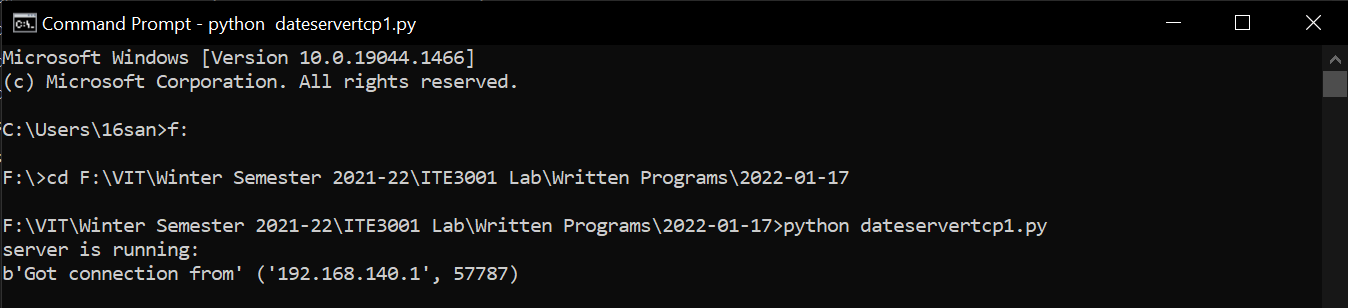
\includegraphics[width=\textwidth]{dateservertcp1.png}
\caption{Server output}
\end{figure}
\begin{figure}[h] % h - Place the float here, i.e., approximately at the same point it occurs in the source text (however, not exactly at the spot)
\centering
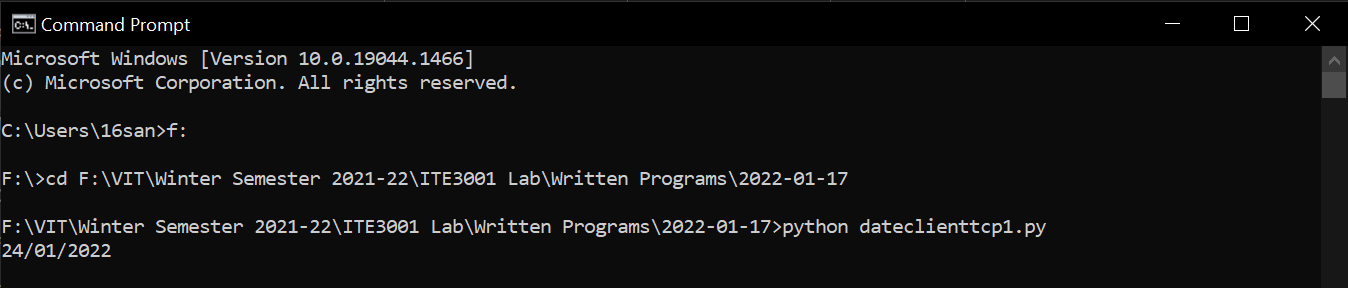
\includegraphics[width=\textwidth]{dateclienttcp1.png}
\caption{Client output}
\end{figure}
\newline
Q2. Write a client-server program, where the client will send a six digit number to the server and the server will add the first, third and fifth position values and the result will be sent back to the client. \newline
Ans- \\ Code- \\ sumservertcp.py-\inputminted{python}{sumservertcp.py}
sumclienttcp.py- \inputminted{python}{sumclienttcp.py}
\newpage
Output-
\begin{figure}[h] % h - Place the float here, i.e., approximately at the same point it occurs in the source text (however, not exactly at the spot)
\centering
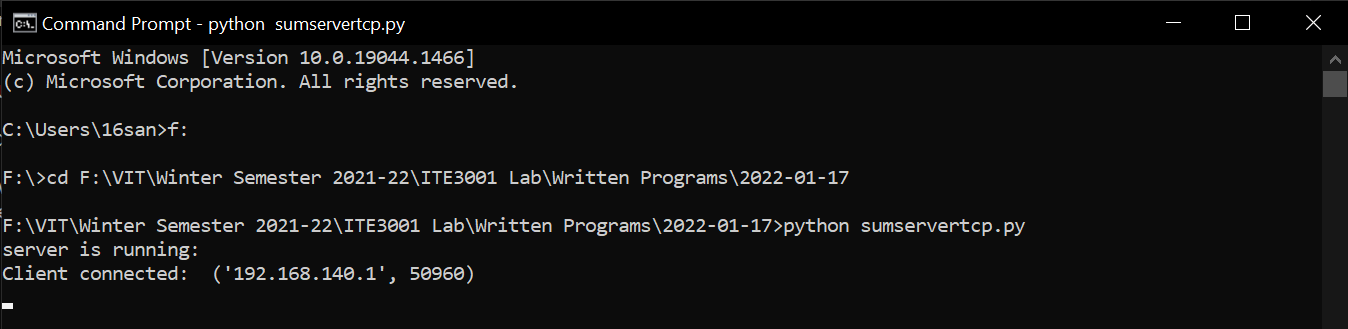
\includegraphics[width=\textwidth]{sumservertcp.png}
\caption{Server output}
\end{figure}
\begin{figure}[h] % h - Place the float here, i.e., approximately at the same point it occurs in the source text (however, not exactly at the spot)
\centering
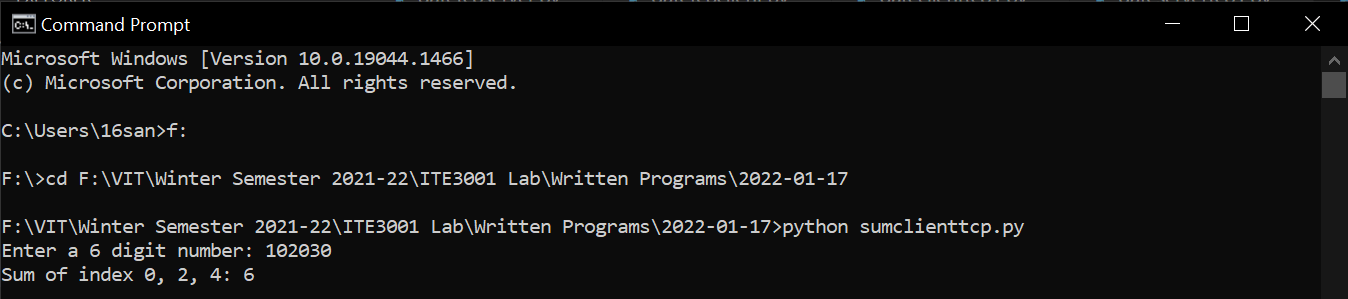
\includegraphics[width=\textwidth]{sumclienttcp.png}
\caption{Client output}
\end{figure}
\newline

Q3. Write a TCP/IP based client-server python code for a “Close Tender”. The tendering process proceeds as follows: The server will think for an amount within 5000-6000 randomly which will be printed as “Proposed Amount” at the server program. Randomly take the “Tender amount” for five users such as User 1, User 2, User 3, User 4 and User 5 in the client side and send those values to the server. The server will compare all user’s value with the “Proposed Amount” to find out the closest one, then, it will send a message “Congratulations!!! (****User name) got the Tender” to the client.\\
Ans- \\ Code- \\ multipleinputserver.py-\inputminted{python}{multipleinputserver.py}
multipleinputclient.py- \inputminted{python}{multipleinputclient.py}
\newpage
Output-
\begin{figure}[h] % h - Place the float here, i.e., approximately at the same point it occurs in the source text (however, not exactly at the spot)
\centering
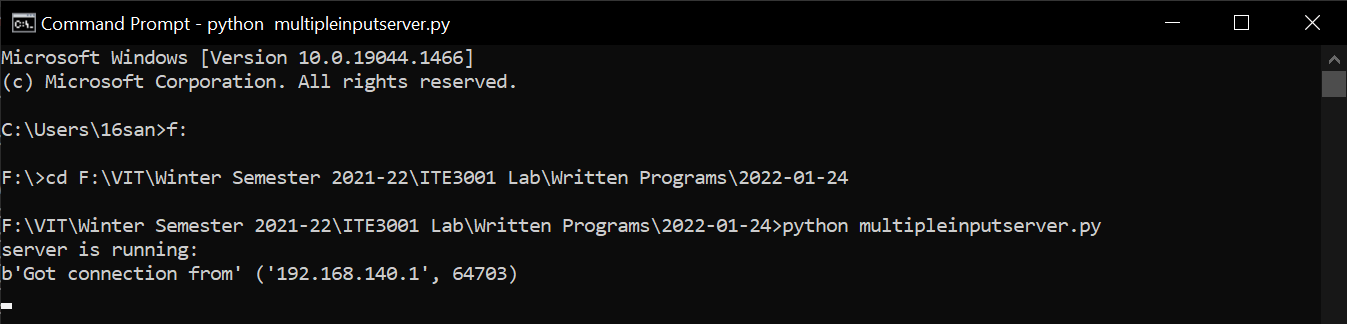
\includegraphics[width=\textwidth]{multipleinputserver.png}
\caption{Server output}
\end{figure}
\begin{figure}[h] % h - Place the float here, i.e., approximately at the same point it occurs in the source text (however, not exactly at the spot)
\centering
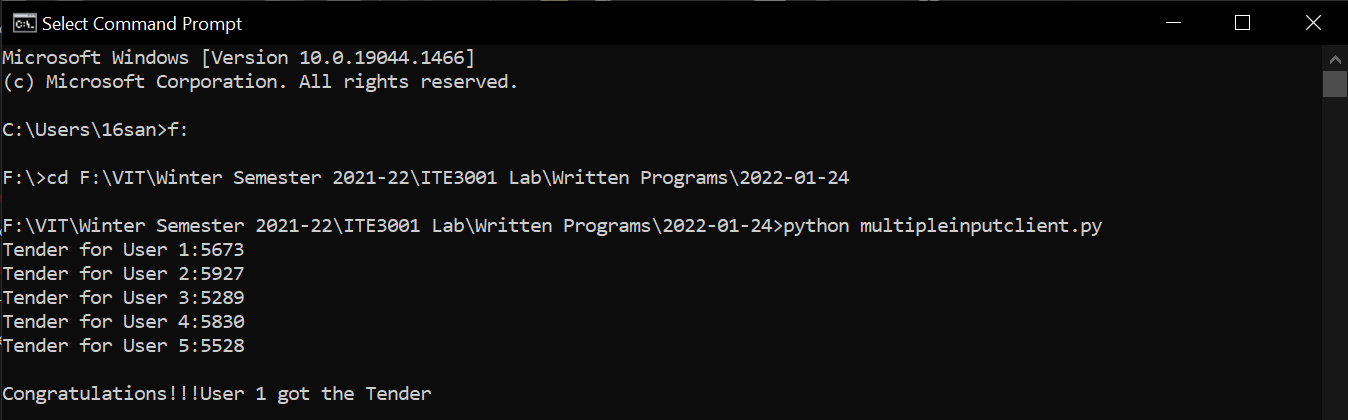
\includegraphics[width=\textwidth]{multipleinputclient.png}
\caption{Client output}
\end{figure}
\end{document}
